The Humboldt Current Ecosystem (HCE) is characterized by a high environmental variability, influencing the distribution and abundance of the main fish stocks. The objective of this thesis was to develop an integrated and multidisciplinary end-to-end (E2E) model of the Northern HCE, including the explicit dynamics of the physical environment, the primary and secondary production, as well as the exploited fish communities. For this purpose, the OSMOSE model was selected to represent the High Trophic Level (HTL) community and an existing application of the ROMS-PISCES hydrodynamic and biogeochemical model for the HCE (Echevin et al. 2012) was selected to represent explicitly the seasonal and interannual forcing from the Low Trophic Level (LTL) community and the physical environment. The interannual effect of fishing was introduced in the OSMOSE model as time series of fishing mortality, which were estimated during the calibration process in order to properly fit the landings data. In the first section of this chapter we start by describing the OSMOSE component model that we had to fully parameterize to represent the dynamics of the HTL community of the NHCE, then briefly describe the ROMS-PISCES model available for the HCE and how its outputs were used to force the OSMOSE model, while in the last section we show how we constructed and validated the spatial maps of the distribution of the modeled species, also used to force OSMOSE. The impact of the interannual variability of fishing and how it is modeled are described in chapter 3.

\section{Modeling the HTL dynamics: OSMOSE}


In OSMOSE, the basic unit of simulation is the ``school'', a group of individuals of the same species sharing the same properties and history in terms of spatial position, length and age. The state of each school in the system can be described by a vector $S = (s, x, y, N, L, A)$, where $s$ is the species the school belongs to, $(x,y)$ is the position of the school (longitude, latitude), $N$ is the number of individuals in the school (abundance), $L$ is the body length of the individuals and $A$ is its age. At any time, the state of the system can be described by the state of all living schools  ($N>0$).
There are three main processes controlling the dynamic of a school: mortality, somatic growth and spatial movement. The core of the first two processes relies in very simple survival and growth assumptions:

\begin{eqnarray}
N(t+1) & = & e^{-Z}N(t)\\
L(t+1) & = & L(t) + G
\end{eqnarray}


In OSMOSE, the total mortality ($Z$) and growth in length ($G$) during a time step are functions of the state of the school itself and that of all other schools in a defined neighbourhood given by the discretization of the spatial domain. This means growth and mortality are function of the state of all schools which are present in the same cell of the grid at the same time. In the OSMOSE version considered in this work, the functions defining mortality and growth are deterministic, while the main source of stochasticity is in the movement process. 

After one time step, each school can move to an adjacent cell of the grid or remain in the same position in a uniform random way. Additionally, the model is forced by species-specific spatial distribution maps. At any time, each school can be assigned to a unique map, while this map can change during the simulation according to age or time-specific criteria (e.g. seasonal maps, different maps for adults or juveniles). When a change in the map for a school occurs, the school is relocated randomly in the new map according to its spatial probability distribution (which can be uniform in the simplest case).

Taken this into account, growth and mortality in OSMOSE depend stochastically on the complex interactions between several schools of different species.
Mortality and growth both depend on the predation process which is length based in OSMOSE. For each species, a school can feed on prey within a limited range of sizes, parameterized by the minimum and maximum ratio between predator and prey sizes. This rule allows each school to ``select'' which other schools it can feed on, considering only the length of the individuals and the co--occurrence in the same cell, so that for most modeled species in the pelagic column, no a priori species-specific trophic relationship is assumed. As a result, the diets, trophic levels and predation mortalities are derived quantities from the model and the size-based predation assumption, and produced as outputs of OSMOSE.

A key parameter linking predation with growth and mortality is the critical predation efficiency threshold $\xi_{max}$, defined as the threshold corresponding to maintenance needs of a fish, and beyond which the food ration can be dedicated to fish growth (Shin and Cury 2001, Shin et al. 2004). This parameter allows correcting the actual growth (no growth below $\xi_{max}$) in the mean length of the school, and adding a starvation mortality $M_\xi$ to the total mortality when predation efficiency is below $\xi_{max}$ (Shin and Cury 2001). 


The size of the fish is modeled by a linear relationship below a critical age or length (fast growth at initial stages, and for which von Bertalanffy growth parameters are usually not well estimated), and beyond that age/size threshold is modeled using the von Bertalanffy model. The actual growth rate (difference in size between two time steps) is calculated on the basis of the von Bertalanffy growth model but taking into account a deviation depending on the predation efficiency at each time step, according to Shin and Cury (2001).


The total mortality for a school is calculated taking into account the food ration needed by co-occurring predator schools (predation mortality), the fishing mortality, the starvation mortality and an additional mortality component $M_0$ representing the mortality due to other processes which are not fully explicit in the model (e.g. due to other predators). The total mortality and its components for each school in the same cell of the grid are solved simultaneously for all species. 

An additional important process leading to the renewal of the population is the reproduction process. Here, the total spawner biomass of each species (aggregated over all schools given a size or age of maturity and sex ratio) leads to an egg production (age 0 abundance). While the recruitment level emerges from the different sources of mortality applied at the subsequent time steps, the initial total egg production is assumed proportional to the spawner biomass, the potential relative fecundity (number of eggs per gram of mature female by unit of time) being the factor of proportionality. These eggs are distributed in a number of new schools proportional to the area of distribution of the species and the expected average biomass of the population for the modeled period. This means that for species with bigger distribution areas, abundance, or both, more new age-0 schools are introduced in the model at each time step. The initial state of the new schools is given by: (i) abundance: the number of eggs after the distribution of the total egg production among all the new schools, (ii) length: the assumed size of the egg for the species, (iii) position: randomly distributed within the age-0 map for the species, and (iv) age 0.

The dynamics of the low trophic level (LTL) species is not explicit in the model, reason why plankton fields (provided by observations or biogeochemical models) are used as forcing variables, representing additional food for planktivorous species or for the smaller species and size classes in OSMOSE. The LTL biomass is available to predation in the same way school biomass is in OSMOSE.

The constants, state variables, parameters, forcings, initial conditions and main derived quantities used in the OSMOSE model are described in Tables \ref{tab:osmose-vars1} and \ref{tab:osmose-vars2}.


\begin{table}
\caption{Description of main quantities used in the OSMOSE model (1).}
\label{tab:osmose-vars1}
\centering \footnotesize 
\begin{tabular}{|p{5cm}|c|c|p{5cm}|}
\hline & Symbol & Units & Remarks\\
\hline \multicolumn{4}{|l|}{1. Constants}\\
\hline Number of low trophic level groups & $N_P$ &&	Species or functional groups from LTL model.\\
\hline Number of species modeled & $N_S$ && Species or functional groups modeled in OSMOSE.\\
\hline Number of age-0 schools & $n^s$ & year$^{-1}$ & Number of new schools per year for species $s$.\\
\hline Number of simulation steps per year	& $N$ &	year$^{-1}$ & \\
\hline Number of simulation years & $T$ & year &  \\
\hline \multicolumn{4}{|l|}{2. State variables}\\	
\hline Number of schools alive & $n^{\#}$ && Schools with positive abundance. \\
\hline Species	& $S$ && $s = 1, \ldots , N_S$\\
\hline Spatial position &	$(x,y)$ & degrees & Position in latitude and longitude.\\
\hline Abundance of the school & $N$ & ind & Number of individuals \\
\hline Average length of individuals of a school & $L$ &cm & \\	
\hline Age of individuals of a school & $A$ & year & \\	
\hline State of a school & $S$ && $S = (s, x, y, N, L, A)$ \\
\hline \multicolumn{4}{|l|}{3. Forcing variables}\\ 
\hline Biomass of plankton from LTL & $B_p(t,x,y)$	& tonnes/km$^2$ & $p = 1, \ldots, N_P$\\
\hline Probability of presence in the habitat & $P_s(t,x,y,a)$ &&	$s = 1, \ldots, N_S$\\
\hline \multicolumn{4}{|l|}{4. Parameters}\\
\hline Critical predation efficiency & $\xi_{max}$ && \\		
\hline Maximum starvation mortality& $M_{\xi,max}^s$ & year$^{-1}$ & \\	
\hline Life history parameters	& $\Phi_s$ && $\Phi_s =~(A_{max}, k, L_{\infty}, t_0, A_{thr}, \newline a, b, l_{egg}, w_{egg}, p_f, L_{50})$, \newline vB equation, length--weight\\
\hline Predation size ratios & $\rho_{s,min}(a,l)$ && $s = 1, \ldots, N_S$\\
& $\rho_{s,max}(a,l)$ && \\
\hline Base natural mortality & $M_s(t,x,y,a,l)$ & year$^{-1}$ & \\	
\hline Fishing mortality &	$F(s,t,x,y,a,l)$ & year$^{-1}$ & \\	
\hline Plankton accessibilities & $\alpha_{p,s}(t)$ && Fraction of plankton group $p$ accessible to predators species $s$ \\
\hline Predation accessibilities & $\alpha_{s,r}(t)$ && Fraction of species group $s$ accessible to predators species $r$ \\
\hline Fecundity & $\varphi^s(t)$ & eggs/tonne/year & \\
\hline Larval mortality & $\lambda^s(t)$ &  month$^{-1}$ & \\	
\hline Inmigration biomass flux & $\psi^s(t)$ & tonnes & \\	
\hline Average length of migratory schools	& $L$ & cm & \\	
\hline Age of migratory schools & $A$ & years & \\	
\hline
\end{tabular} 
\end{table}


\begin{table}
\caption{Description of main quantities used in the OSMOSE model (2).}
\label{tab:osmose-vars2}
\centering \footnotesize 
\begin{tabular}{|p{5cm}|c|c|p{4cm}|}
\hline & Symbol & Units & Remarks\\
\hline \multicolumn{4}{|l|}{5. Derived quantities}\\
\hline Spatial distribution of abundance & $N_s(t, x, y)$ & ind/km$^2$ & $s = 1, \ldots, N_S$ \\
Spatial distribution of biomass & $B_s(t, x, y)$ & tonnes/km$^2$ & \\	
\hline Total abundance of the population &  $N_s(t)$ & ind & \\
Total biomass of the population & $B_s(t)$ & tonnes & \\	
\hline Catch-at-age & $C_s(t, a)$ & ind  & \\
Catch-at-length & $C_s(t, l)$ &&\\
\hline Yield & $Y_s(t, x, y)$ & tonnes/km$^2$ & \\	
\hline Total yield	& $Y_s(t)$ &tonnes & \\	
\hline Predation mortality & $P_{s,r}(t, x, y)$ && Prey $s = 1, \ldots, N_S$ \\
Starvation mortality & $M_\xi(s, t, x, y)$ & year$^{-1}$ & Predator $r = 1, \ldots, N_S$\\
Total mortality	& $Z(s, t, x, y)$ && \\ 
\hline Trophic level & $TL(s,t,x,y,l)$ && \\		
\hline \multicolumn{4}{|l|}{6. Initial conditions}\\
\hline Total biomass & $B_0^s$ & tonnes & \\	
\hline School states & $S_0^i = (s, x, y, l, a)$ && $i = 1, \ldots,n_0^\#$.\\
\hline
\end{tabular} 
\end{table}

\section{Interannual forcing of the plankton: ROMS--PISCES}


ROMS (Regional Oceanic Modeling System, Shchepetkin and McWilliams 2005) is a free surface ocean model that solves the primitive equations of oceandynamics. Widely used by the scientific community in a diverse range of applications in the world (Haidvogel et al 2000, Peliz et al 2003, Di Lorenzo 2003, Dinniman et al. 2003, Budgell 2005, Warner et al. 2005a, 2005b, Wilkin et al. 2005), it has been especially designed to produce realistic simulations of the dynamics of regional systems. 

The PISCES (Pelagic Interaction Scheme for Carbon and Ecosystem Studies) biogeochemical model simulates marine biological productivity and describes biogeochemical cycles of carbon and major nutrients in the ocean (Aumont and Bopp 2006). PISCES assumes that phytoplankton growth depends on external concentration of nutrients and that the main nutrients in the medium follow the Redfield ratio (C:N:P $\sim$ 106:16:1) (Redfield et al 1963). PISCES has 24 state variables, among which are nutrients (Phosphorus, Nitrogen, Silica and Iron), dissolved oxygen, two kinds of detritus (large and small), two classes of zooplankton (microzooplankton and mesozooplankton) and two kinds of phytoplankton (nanophytoplankton and diatoms). Diatoms differ from nanophytoplankton in their requirements in silicates, an increased consumption of iron and higher levels of saturation due to its larger size (Echevin et al. 2008).

\subsection{ROMS--PISCES model setup}

In Peru, there have been several modeling studies of climatological variability (Penven et al. 2005, Montes et al. 2010) and the effects of El Niño 1997-1998 (Colas et al. 2008). 

However, the simulations used in this thesis are the first that investigate a period over 15 years (1992-2008) in an area corresponding to the Southeast Pacific delimited between 100º and 70º W and 10º N to 40º S, covering a larger area to the north than the HCE to reproduce more accurately the equatorial circulation, because changes in the dynamics of equatorial currents (surface and subsurface) would influence directly the dynamics (Montes et al. 2010), richness, oxygenation and productivity (Espinoza-Morriberón 2012) of the waters off Peru. In the present study the PISCES model is coupled to the physical model ROMS, following the approach of Gruber et al. (2006), who coupled ROMS to a simpler biogeochemical model than PISCES. The spatial resolution is 1/6º with 32 sigma vertical levels (which follow the topography of the ocean floor). Atmospheric forcings were constructed from: i) binding of climatological SCOW data (Risien and Chelton 2008) with NCEP anomalies (\url{www.ncep.noaa.gov}) for wind fields and, ii) binding of COADS climatology data (Da Silva et al. 1994) with NCEP anomalies for the heat fluxes and air temperatures. For boundary conditions the outputs of the global simulation of the ORCA2-PISCES physical-biogeochemical coupled model (Aumont and Bopp 2006) were used, and they were forced with NCEP data. For more information about the construction of simulation forcings and boundaries, the reader can refer to Echevin et al. (2012), Cambon et al. (2013) and the webpage of the project ``Peru Ecosystem Projection Scenarios (PEPS)'' (\url{www.locean-ipsl.upmc.fr/PEPS}).

\subsection{Coupling ROMS--PISCES with the OSMOSE model}

The results of this ROMS-PISCES simulation were validated through its ability to represent the climatological and interannual variability from 1992 to 2008 (Romero et al. submitted, Espinoza et al. submitted) of the main physical variables corresponding to the South East Pacific ocean region (temperature, salinity, currents and sea level),the distribution of surface water masses, the depth of the oxygen minimum zone (OMZ), as well as concentrations of nutrients and surface chlorophyll-a.  

The concentration fields of the four groups of plankton modeled in PISCES (nanophytoplankton, diatoms, microzooplankton and mesozooplankton) are used as prey fields forcing the OSMOSE model, where planktivorous fish can have access to the plankton according to the size-based predation rules implemented in the model. Additionally, the depth of the oxygen minimum zone is used as a predictor of the spatial distribution of all the modeled species as described in the next section.

\begin{figure}
\centering
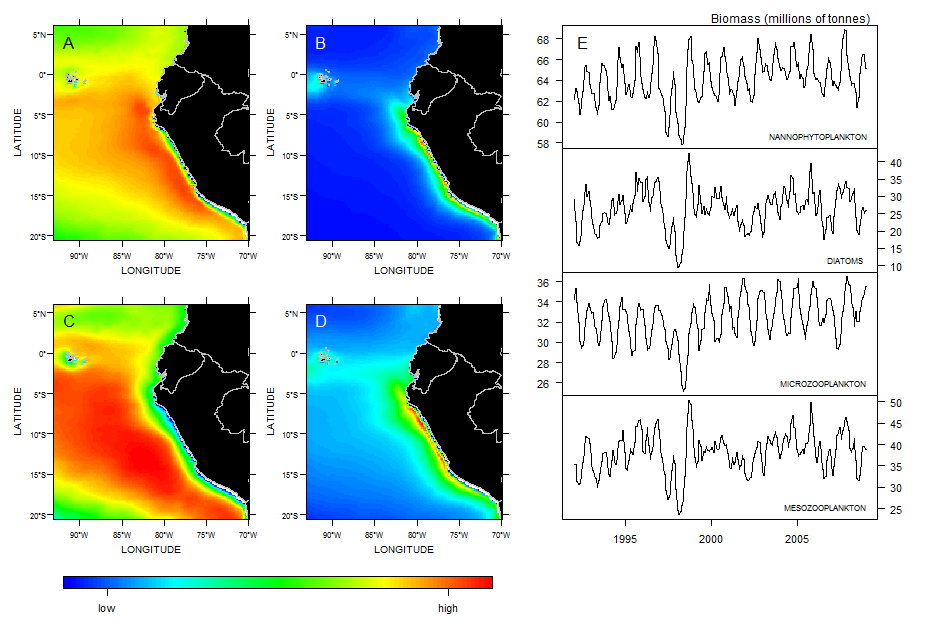
\includegraphics[width=0.95\linewidth]{figures/figuraA1}
\caption{Summary of the LTL biomass simulated by ROMS-PISCES model used as forcing for OSMOSE. Average spatial distribution for nanophytoplankton (A), diatoms (B), microzooplankton (C) and mesozooplankton (D) (red is high, blue is low, following the light visible spectrum). Simulated temporal dynamics of thetotal biomass (millions of tonnes) of the four plankton groups (E) is also shown.}
\label{fig:figureA1}
\end{figure}



\section{Modelling the variability in fish habitat distribution}

In order to model the interannual variability in the distribution of the species included in the NHCE OSMOSE model, several GAM models were constructed. A more detailed description of the model building and validation for Jack mackerel is presented here, highlighting some of the issues we found when constructing time series of maps. The results for other species are shown thereafter.

\subsection[Pattern--oriented validation of habitat distribution models]{Pattern-oriented validation of habitat distribution models}

The following manuscript is in preparation for submission as a short communication to the ICES Journal of Marine Science.

\includepaper{figures/Oliveros_etal-validation_niche_models-for_print.pdf}


\subsection{Prediction of the spatial distribution of modeled fish in the NHCE} 

Similar models and methods as described in the previous subsection for Jack mackerel were applied to the other species explicitly modeled in OSMOSE (macrozooplankton, anchovy, sardine, chub mackerel, mesopelagic fish, red lobster or munida, jumbo squid and the Peruvian hake). The seasonal patterns of the distribution as a summary of these results are shown in the next figures.

\begin{figure}
\centering
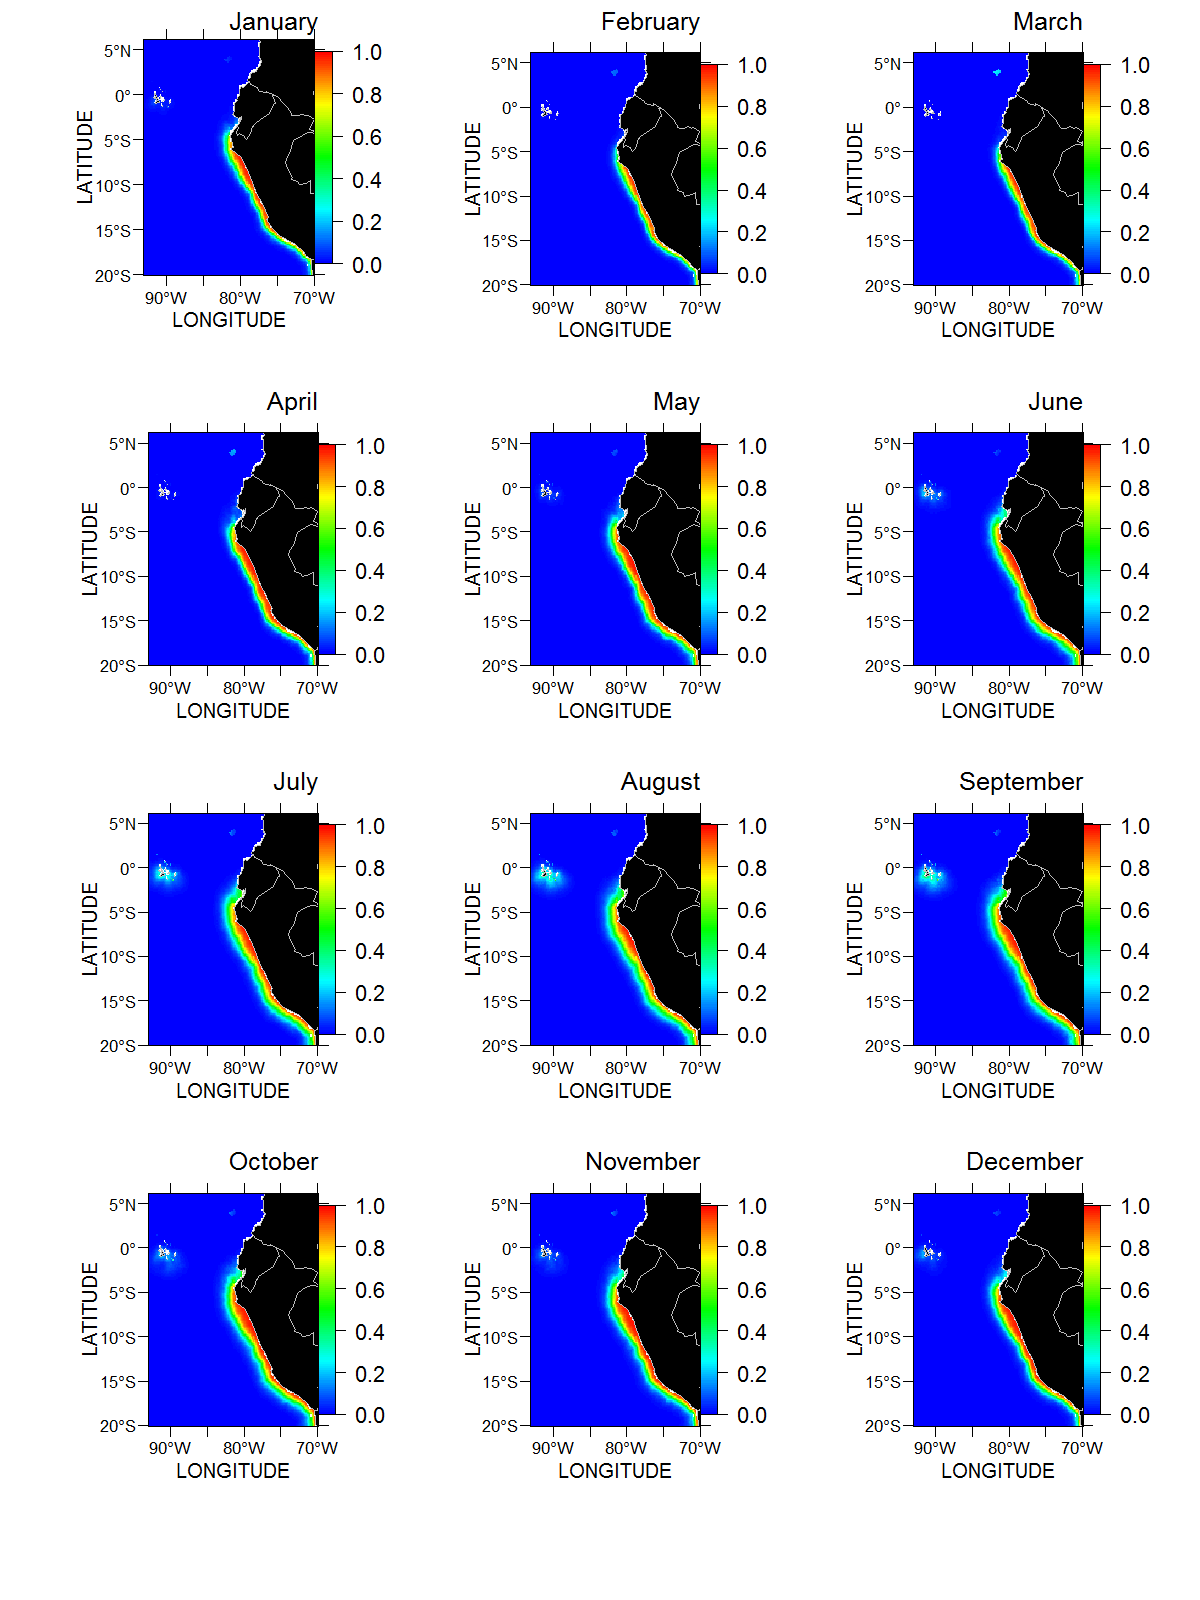
\includegraphics[height=0.8\textheight]{figures/anchovy-climatology}
\caption[Seasonal patterns of the distribution of Peruvian anchovy]{Seasonal patterns of the distribution of Peruvian anchovy as predicted by the species distribution models used to build the interannual maps for the NHCE OSMOSE model.}
\label{fig:anchovy-climatology}
\end{figure}

\begin{figure}
\centering
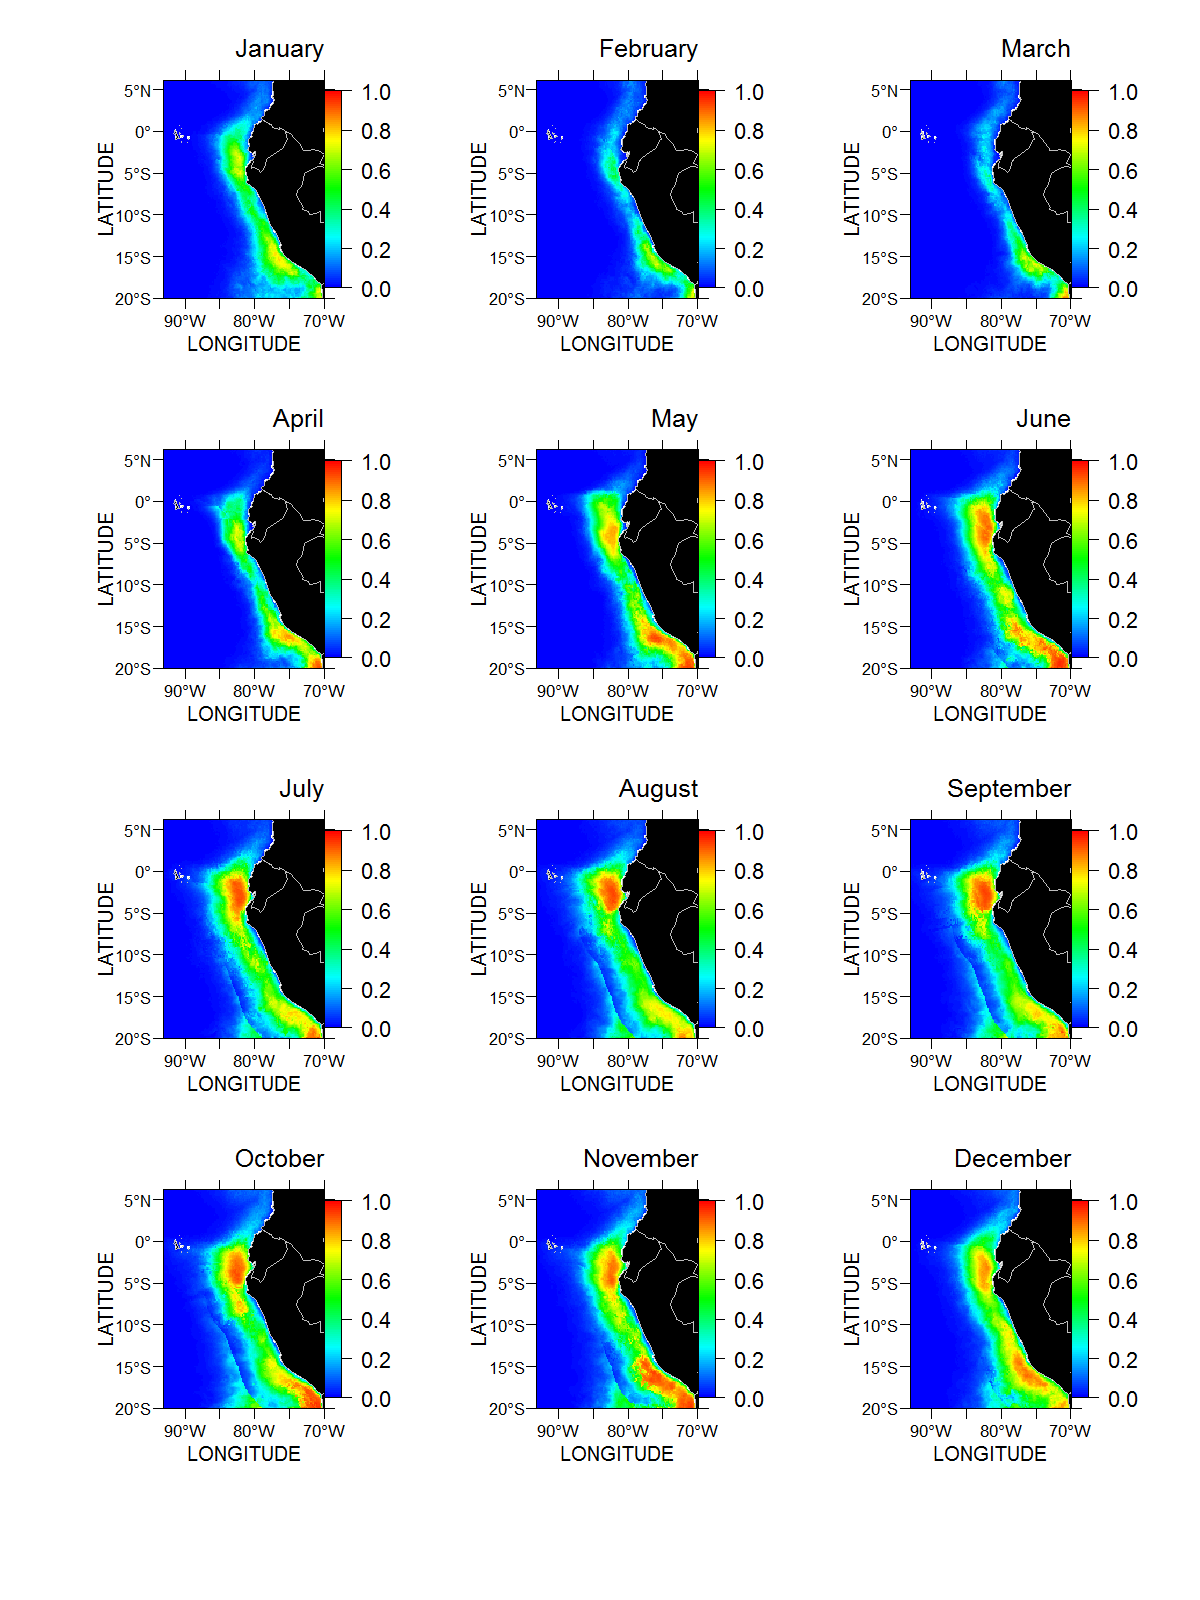
\includegraphics[height=0.8\textheight]{figures/jurel-climatology}
\caption[Seasonal patterns of the distribution of Jack mackerel]{Seasonal patterns of the distribution of Jack mackerel as predicted by the species distribution models used to build the interannual maps for the NHCE OSMOSE model.}
\label{fig:jurel-climatology}
\end{figure}

\begin{figure}
\centering
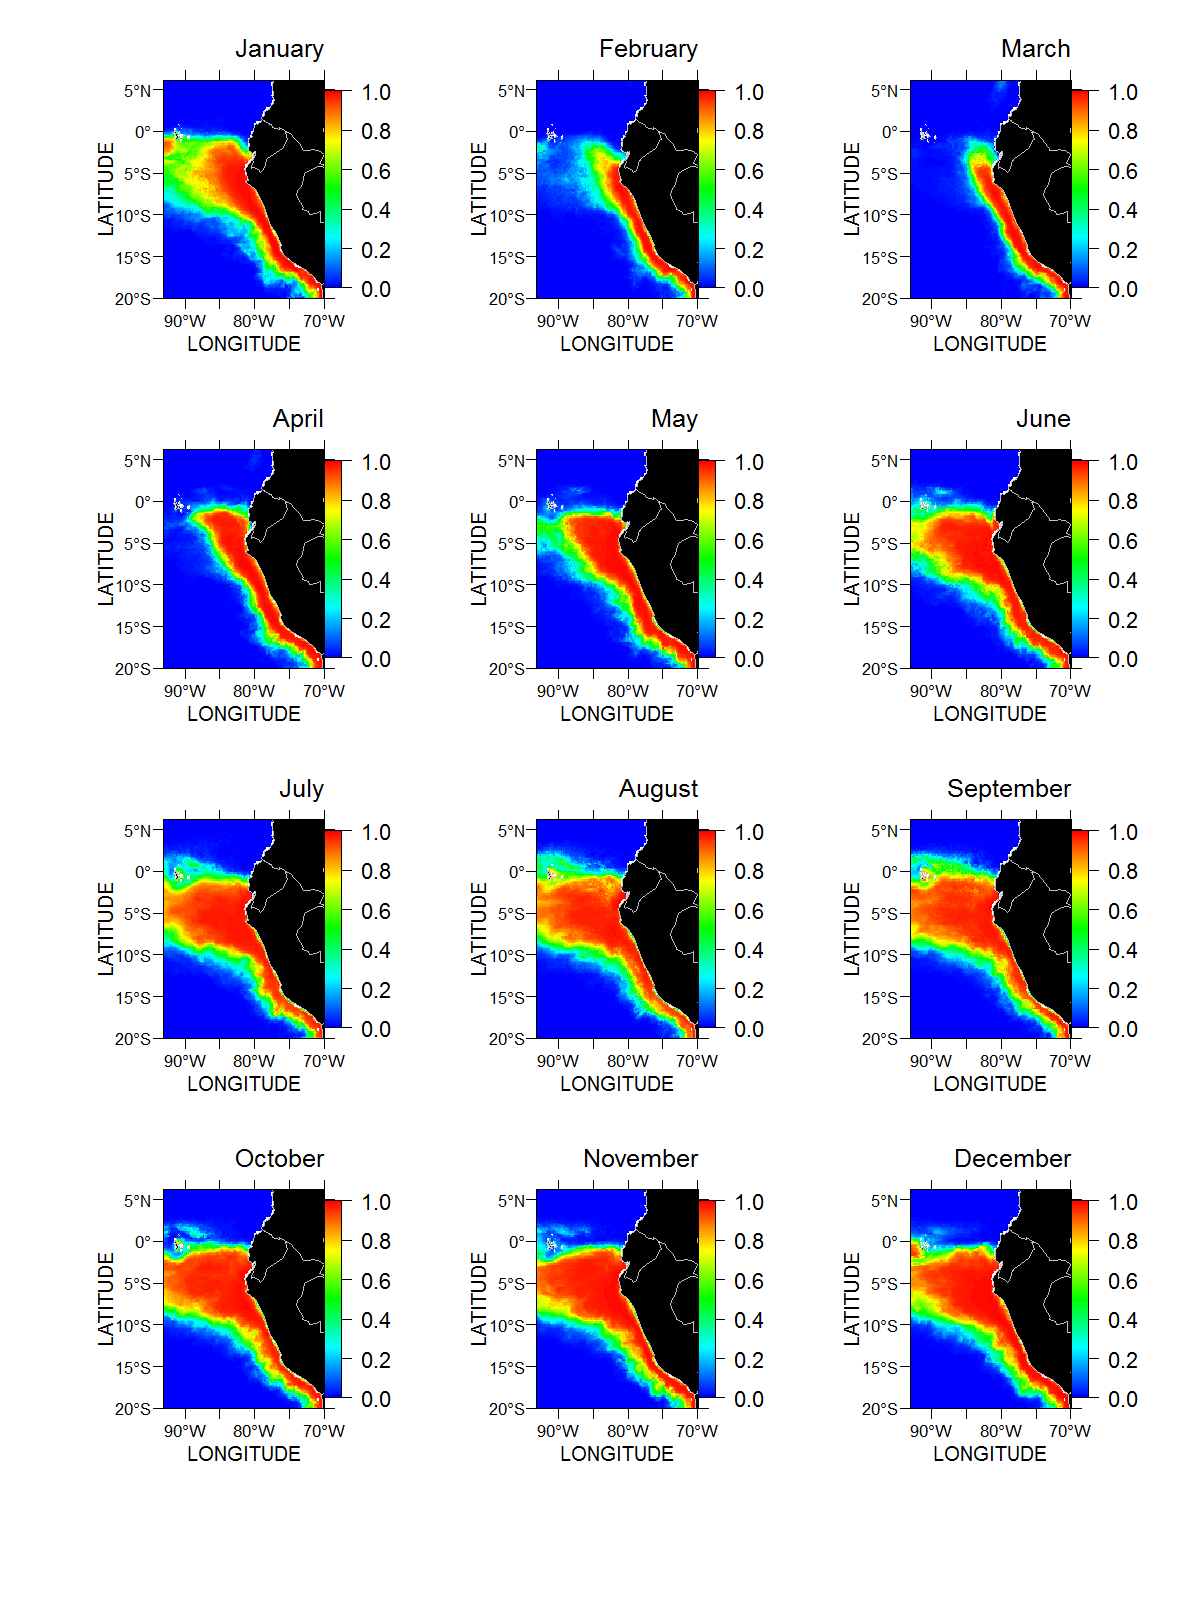
\includegraphics[height=0.8\textheight]{figures/euphausidos-climatology}
\caption[Seasonal patterns of the distribution of Macrozooplankton]{Seasonal patterns of the distribution of macrozooplankton as predicted by the species distribution models used to build the interannual maps for the NHCE OSMOSE model.}
\label{fig:euphausidos-climatology}
\end{figure}

\begin{figure}
\centering
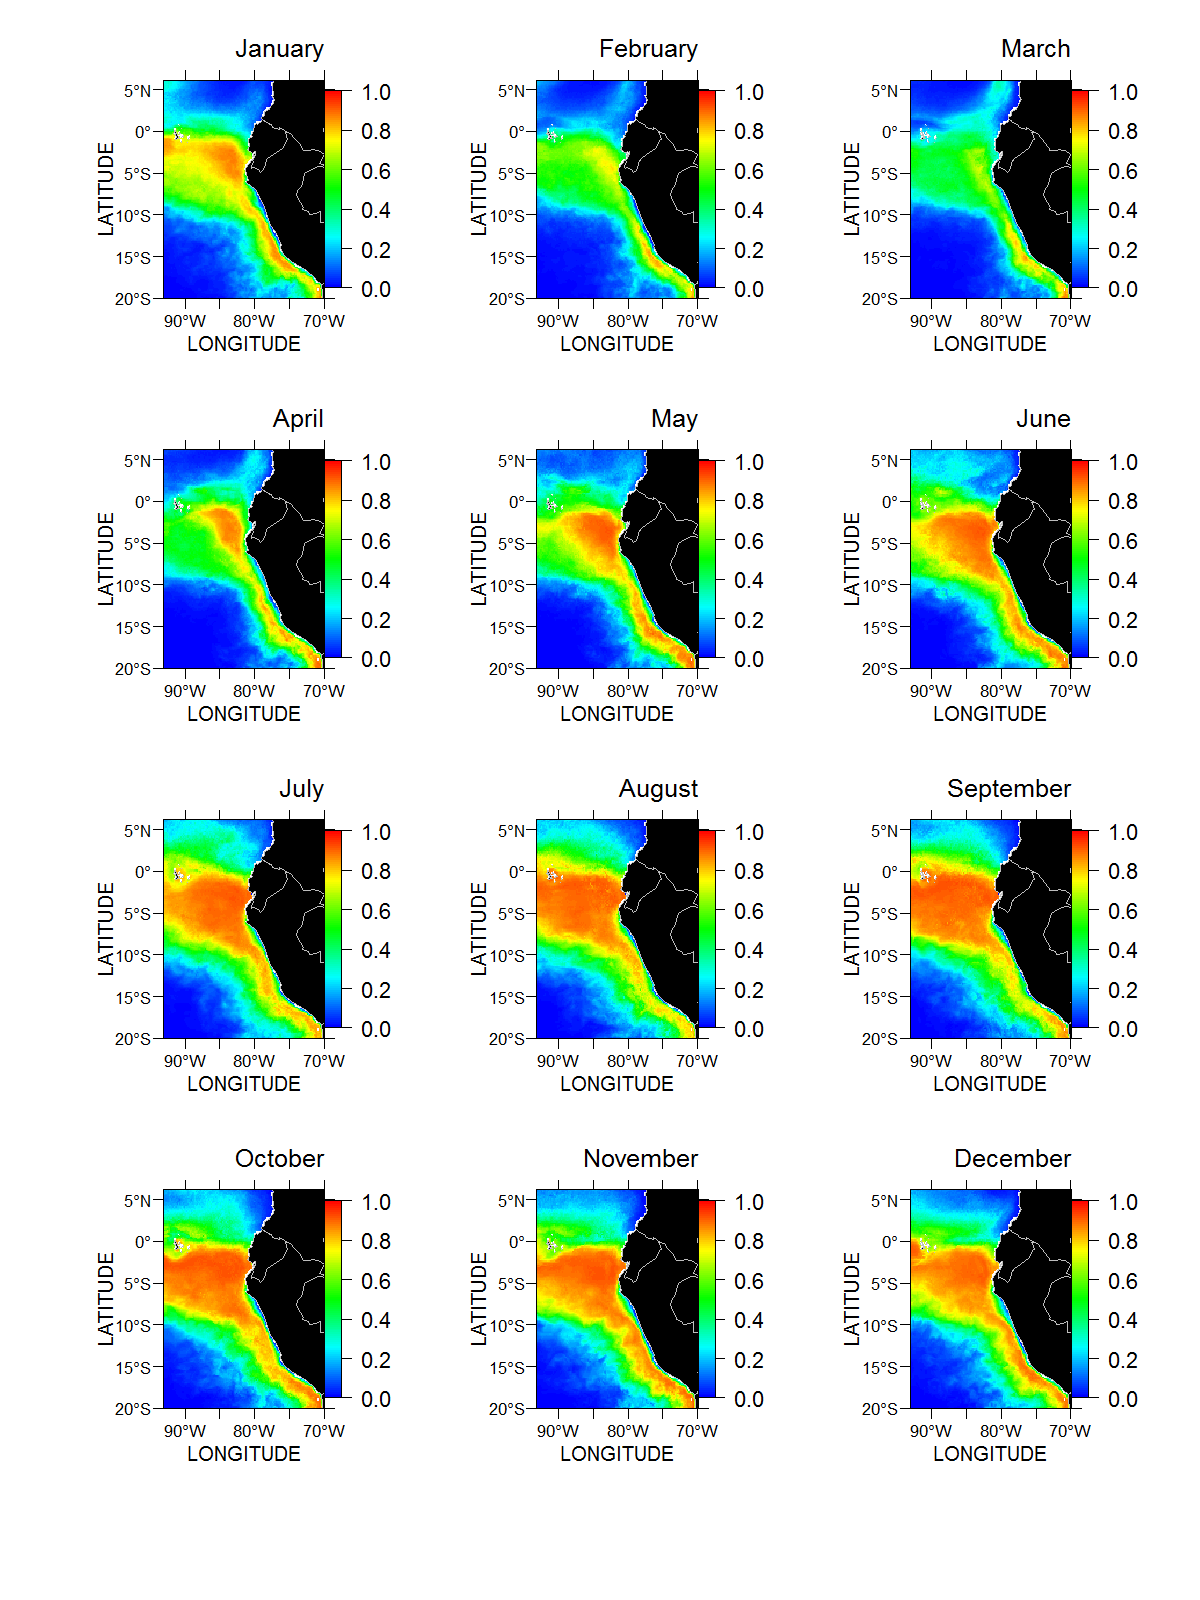
\includegraphics[height=0.8\textheight]{figures/pota-climatology}
\caption[Seasonal patterns of the distribution of Humboldt squid]{Seasonal patterns of the distribution of Humboldt squid as predicted by the species distribution models used to build the interannual maps for the NHCE OSMOSE model.}
\label{fig:pota-climatology}
\end{figure}

\begin{figure}
\centering
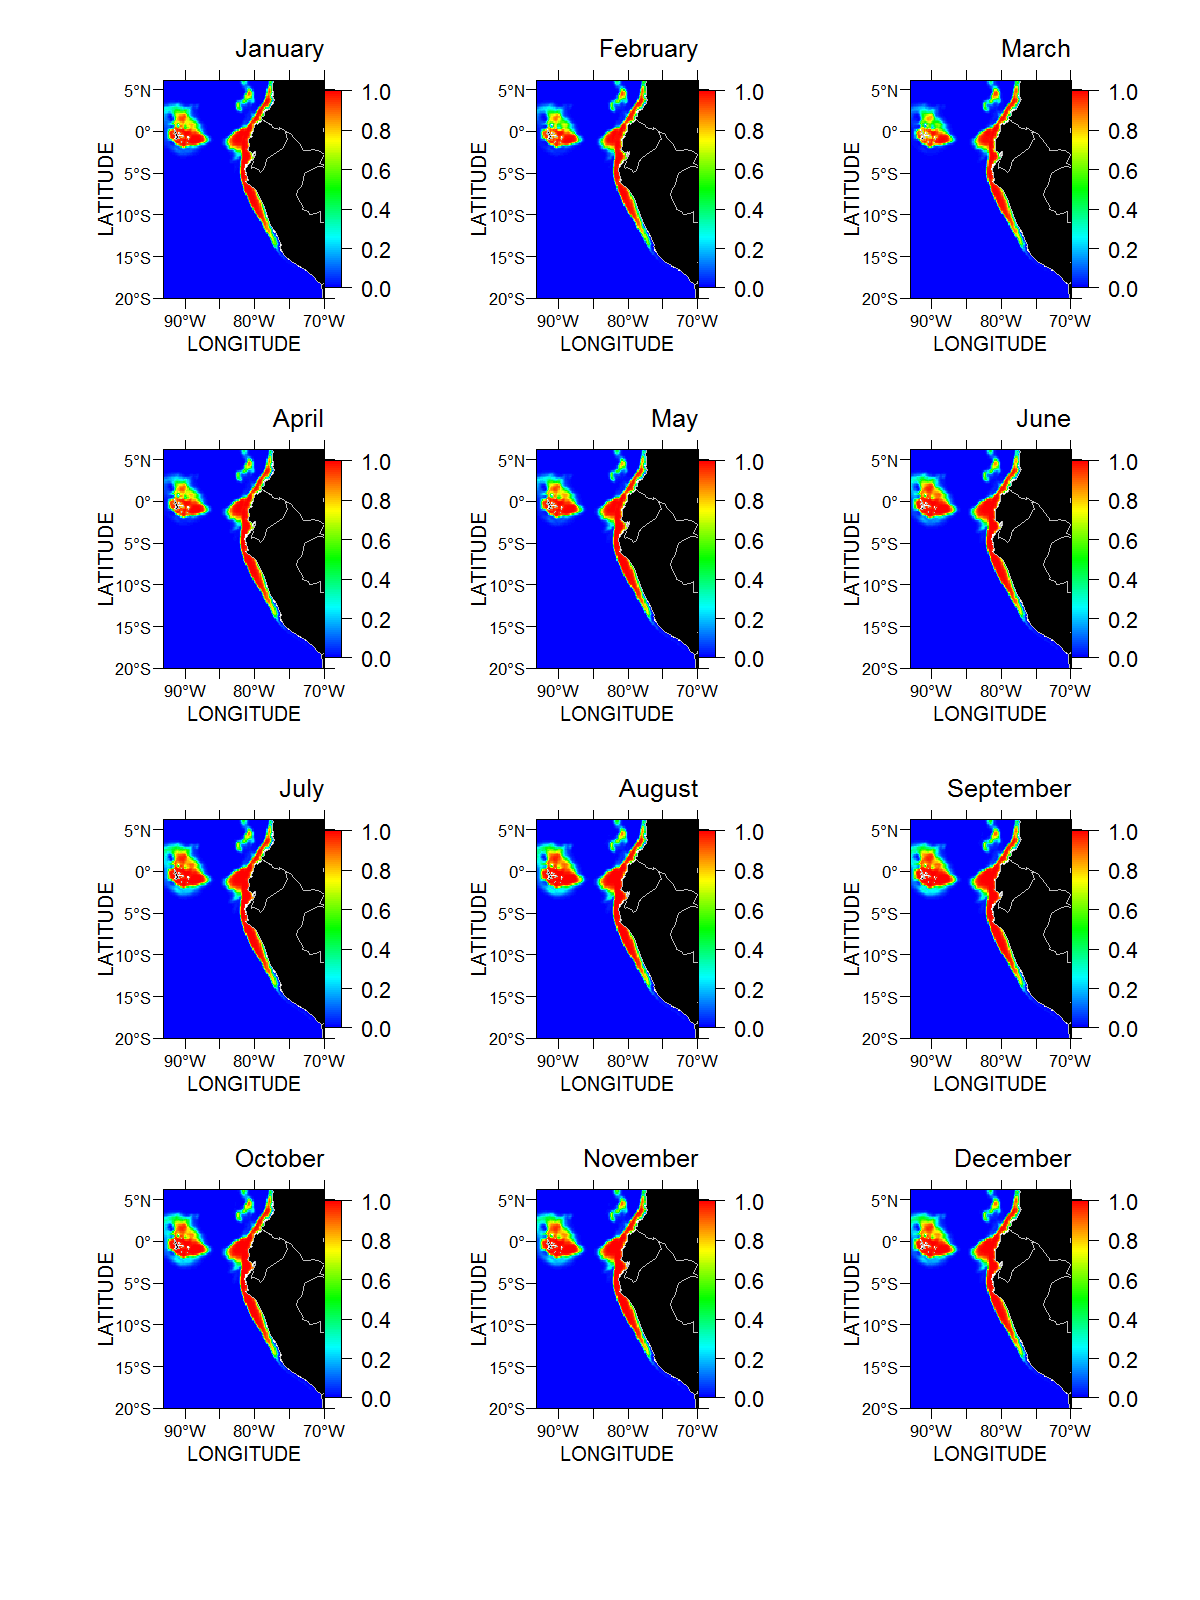
\includegraphics[height=0.8\textheight]{figures/hake-climatology}
\caption[Seasonal patterns of the distribution of Peruvian hake]{Seasonal patterns of the distribution of Peruvian hake as predicted by the species distribution models used to build the interannual maps for the NHCE OSMOSE model.}
\label{fig:hake-climatology}
\end{figure}

\begin{figure}
\centering
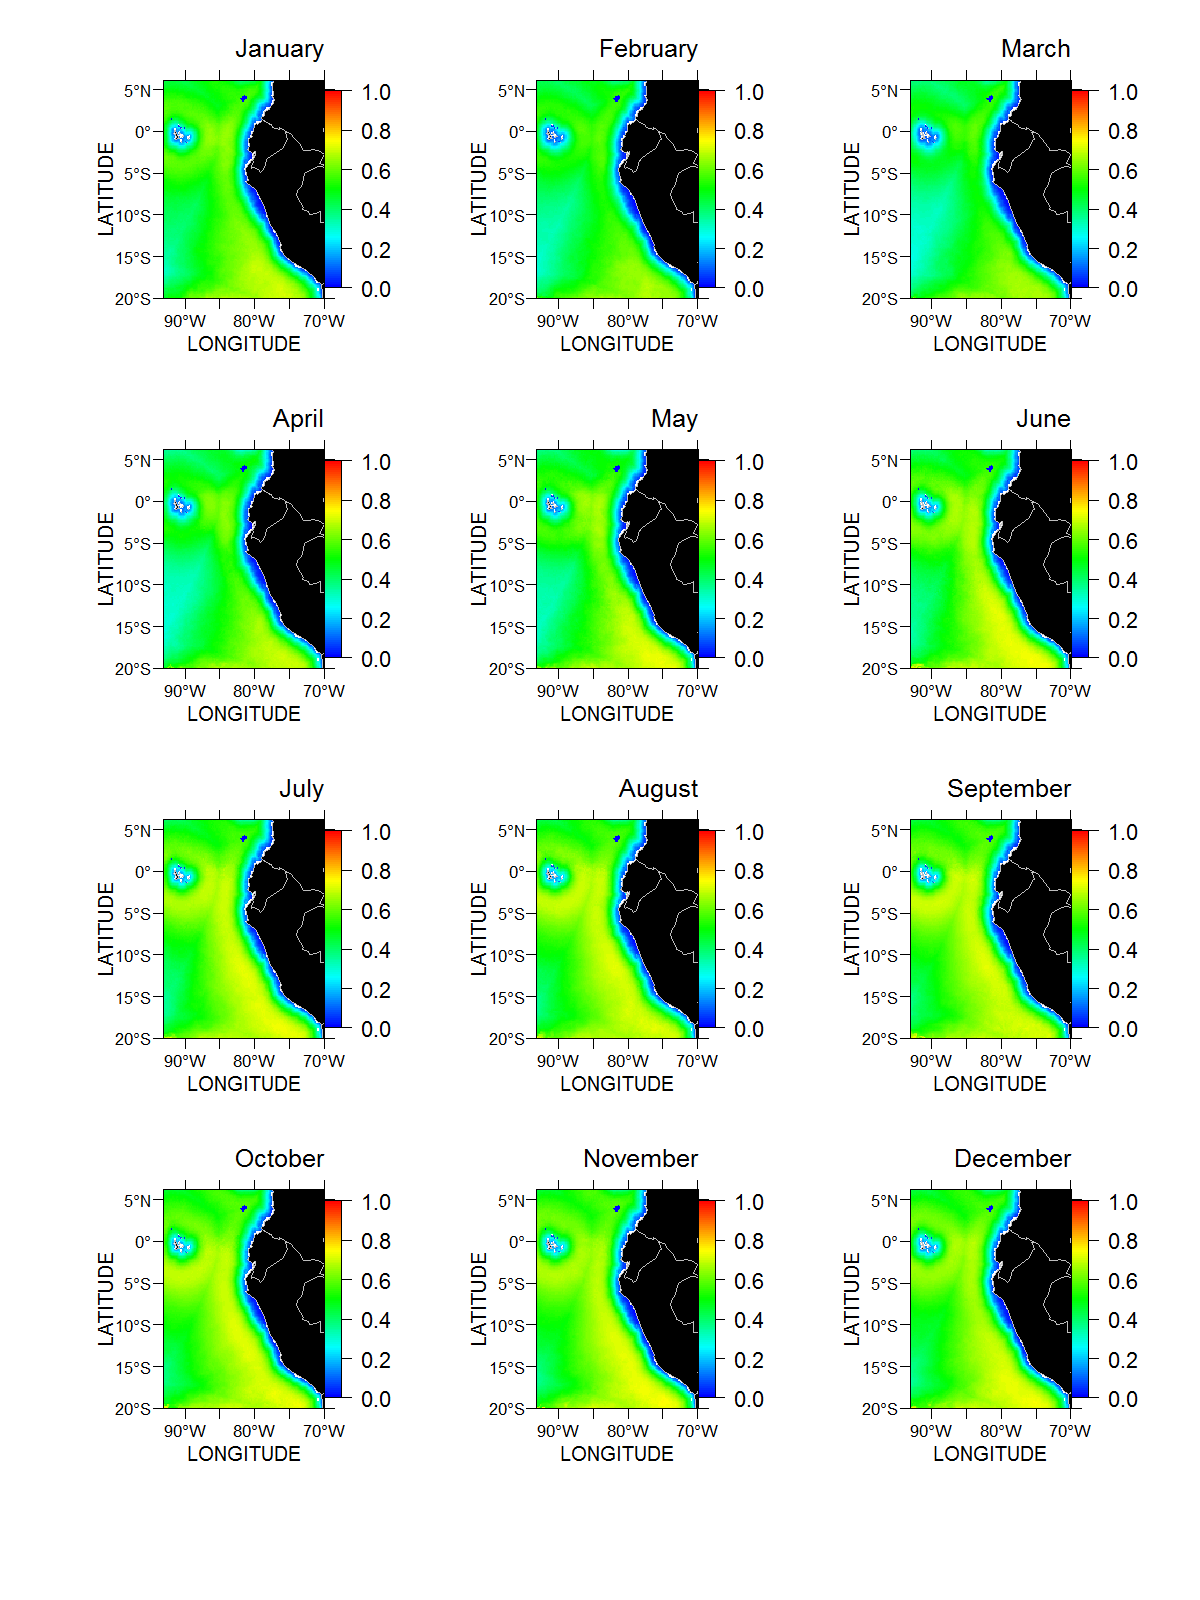
\includegraphics[height=0.8\textheight]{figures/meso-climatology}
\caption[Seasonal patterns of the distribution of mesopelagic fish]{Seasonal patterns of the distribution of mesopelagic fish as predicted by the species distribution models used to build the interannual maps for the NHCE OSMOSE model.}
\label{fig:meso-climatology}
\end{figure}

\begin{figure}
\centering
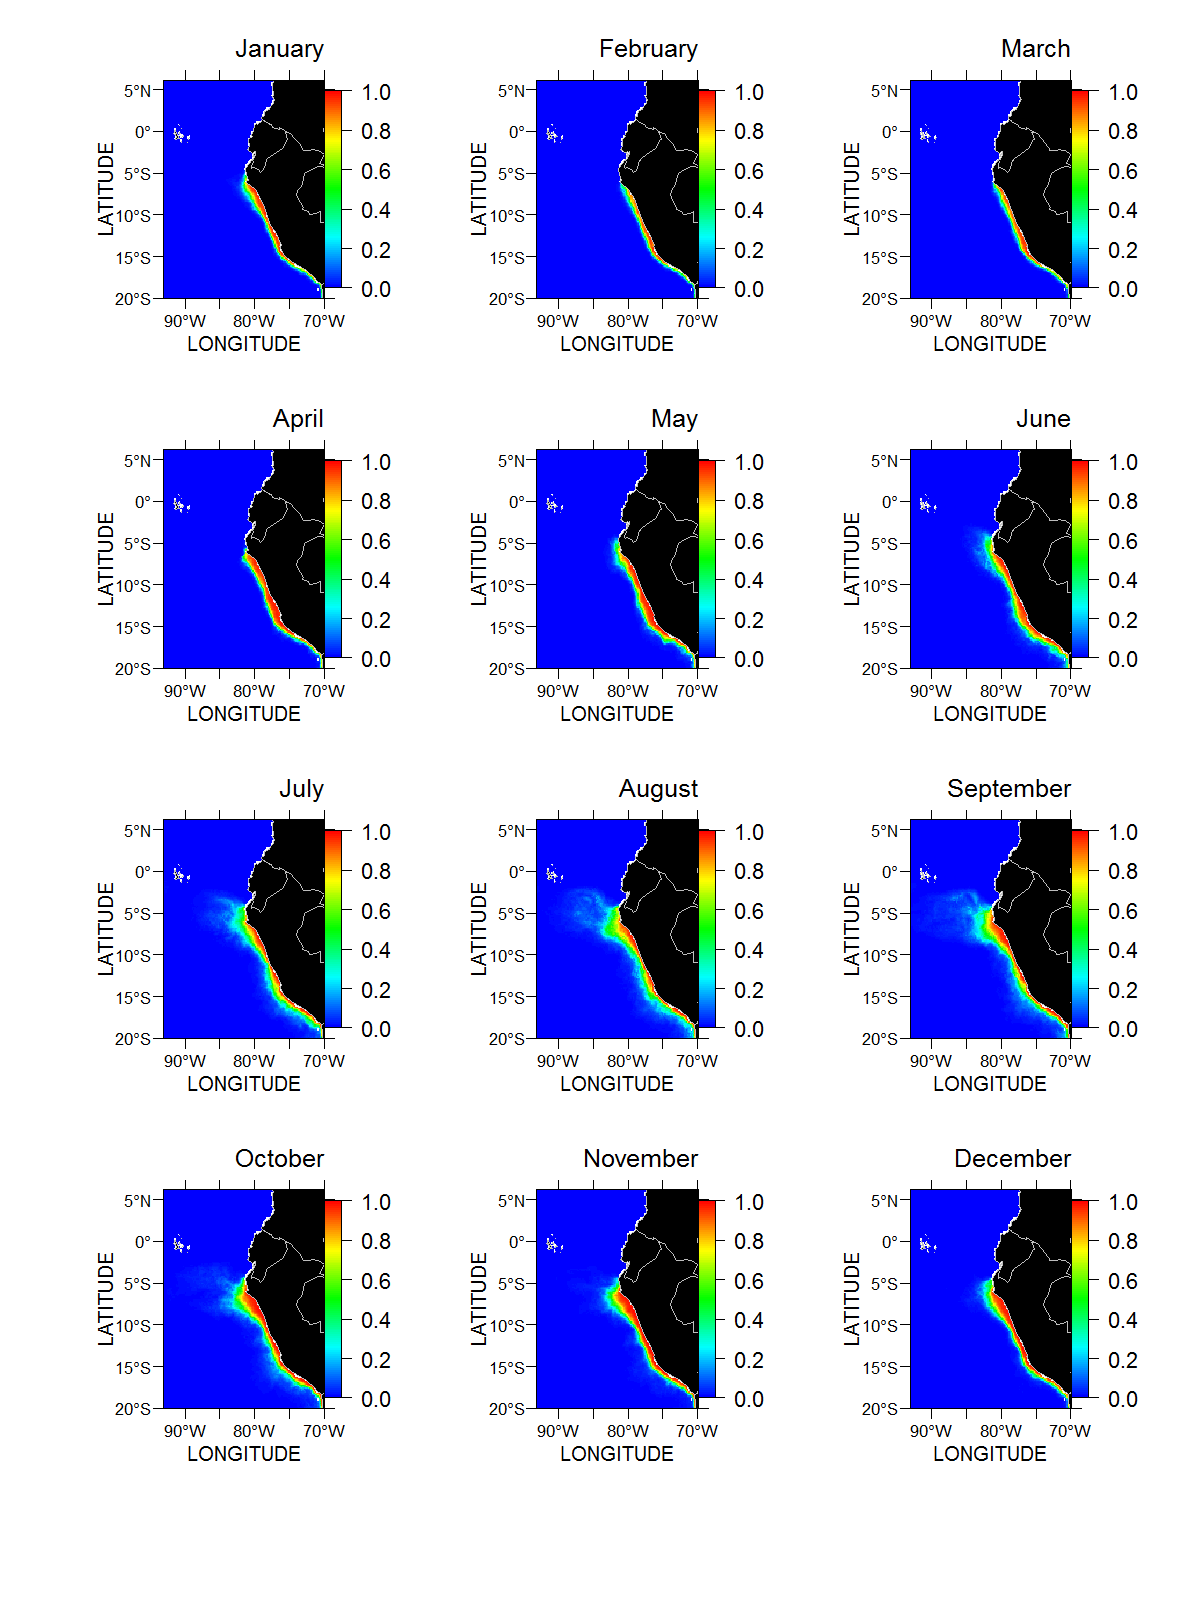
\includegraphics[height=0.8\textheight]{figures/munida-climatology}
\caption[Seasonal patterns of the distribution of Munida]{Seasonal patterns of the distribution of Munida as predicted by the species distribution models used to build the interannual maps for the NHCE OSMOSE model.}
\label{fig:munida-climatology}
\end{figure}

\begin{figure}
\centering
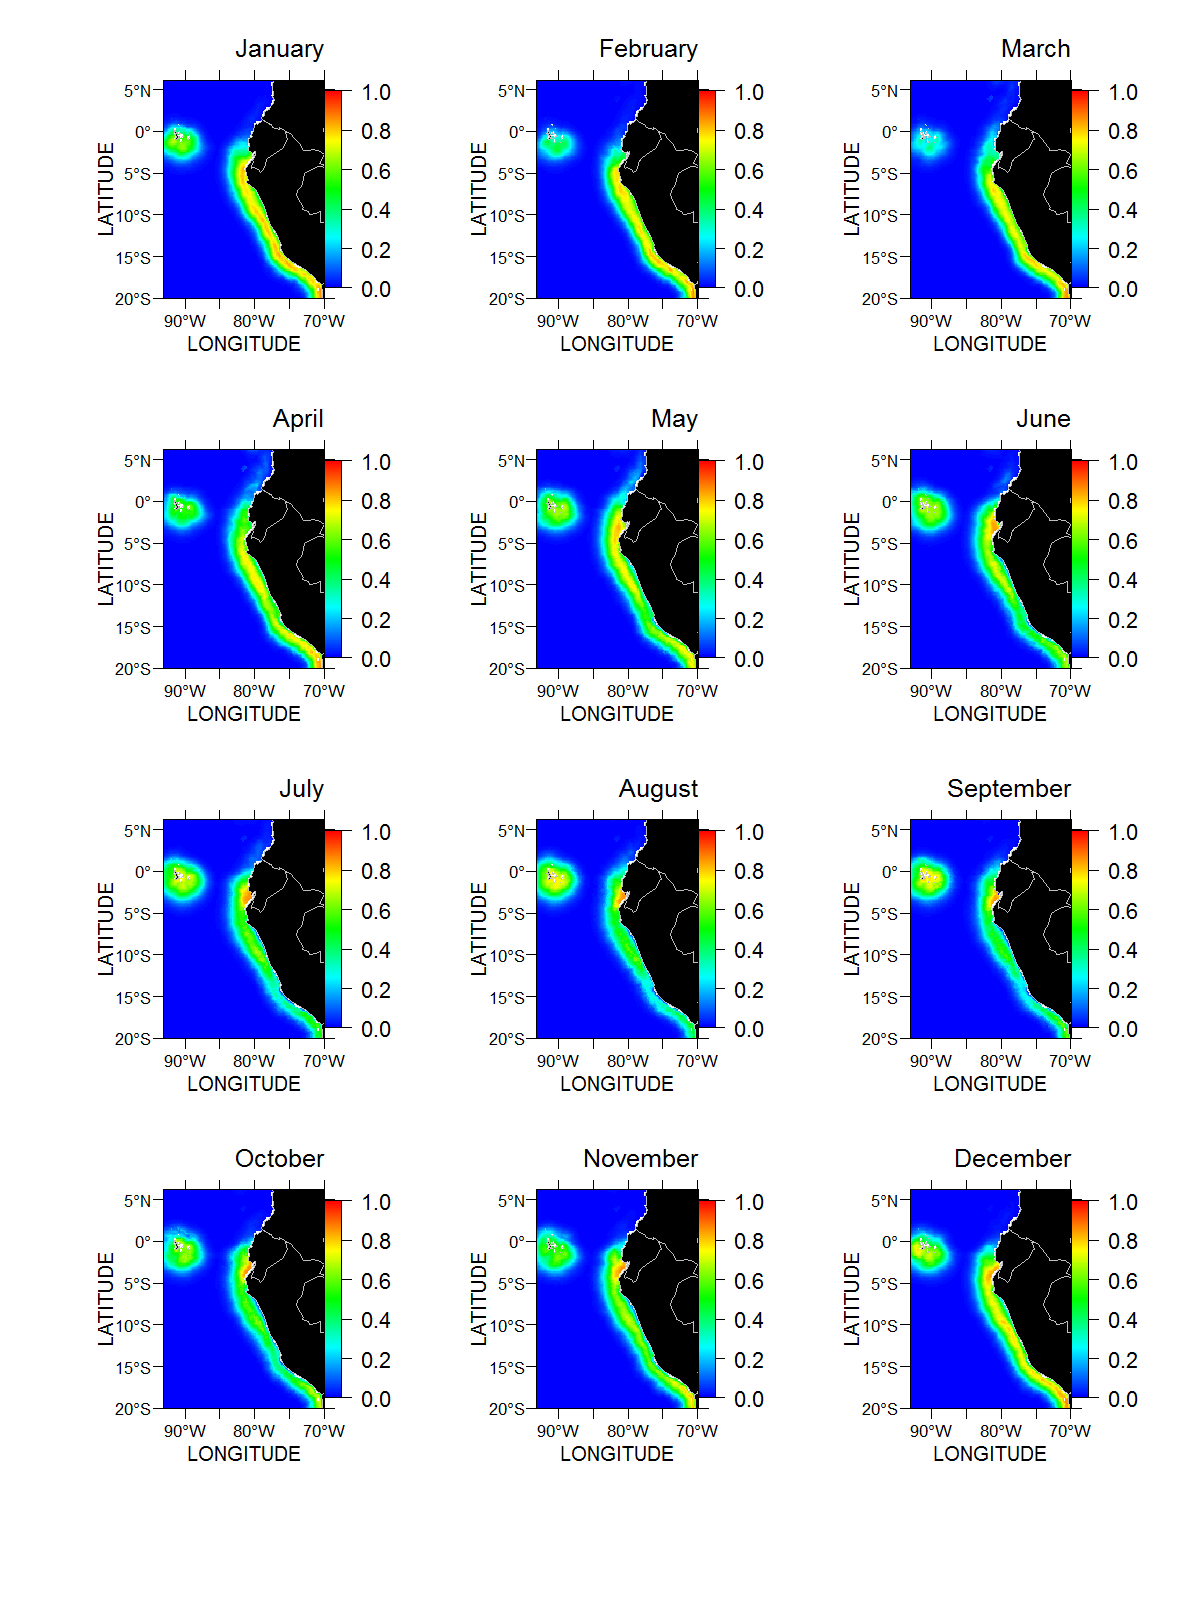
\includegraphics[height=0.8\textheight]{figures/caballa-climatology}
\caption[Seasonal patterns of the distribution of mackerel]{Seasonal patterns of the distribution of mackerel as predicted by the species distribution models used to build the interannual maps for the NHCE OSMOSE model.}
\label{fig:caballa-climatology}
\end{figure}

\begin{figure}
\centering
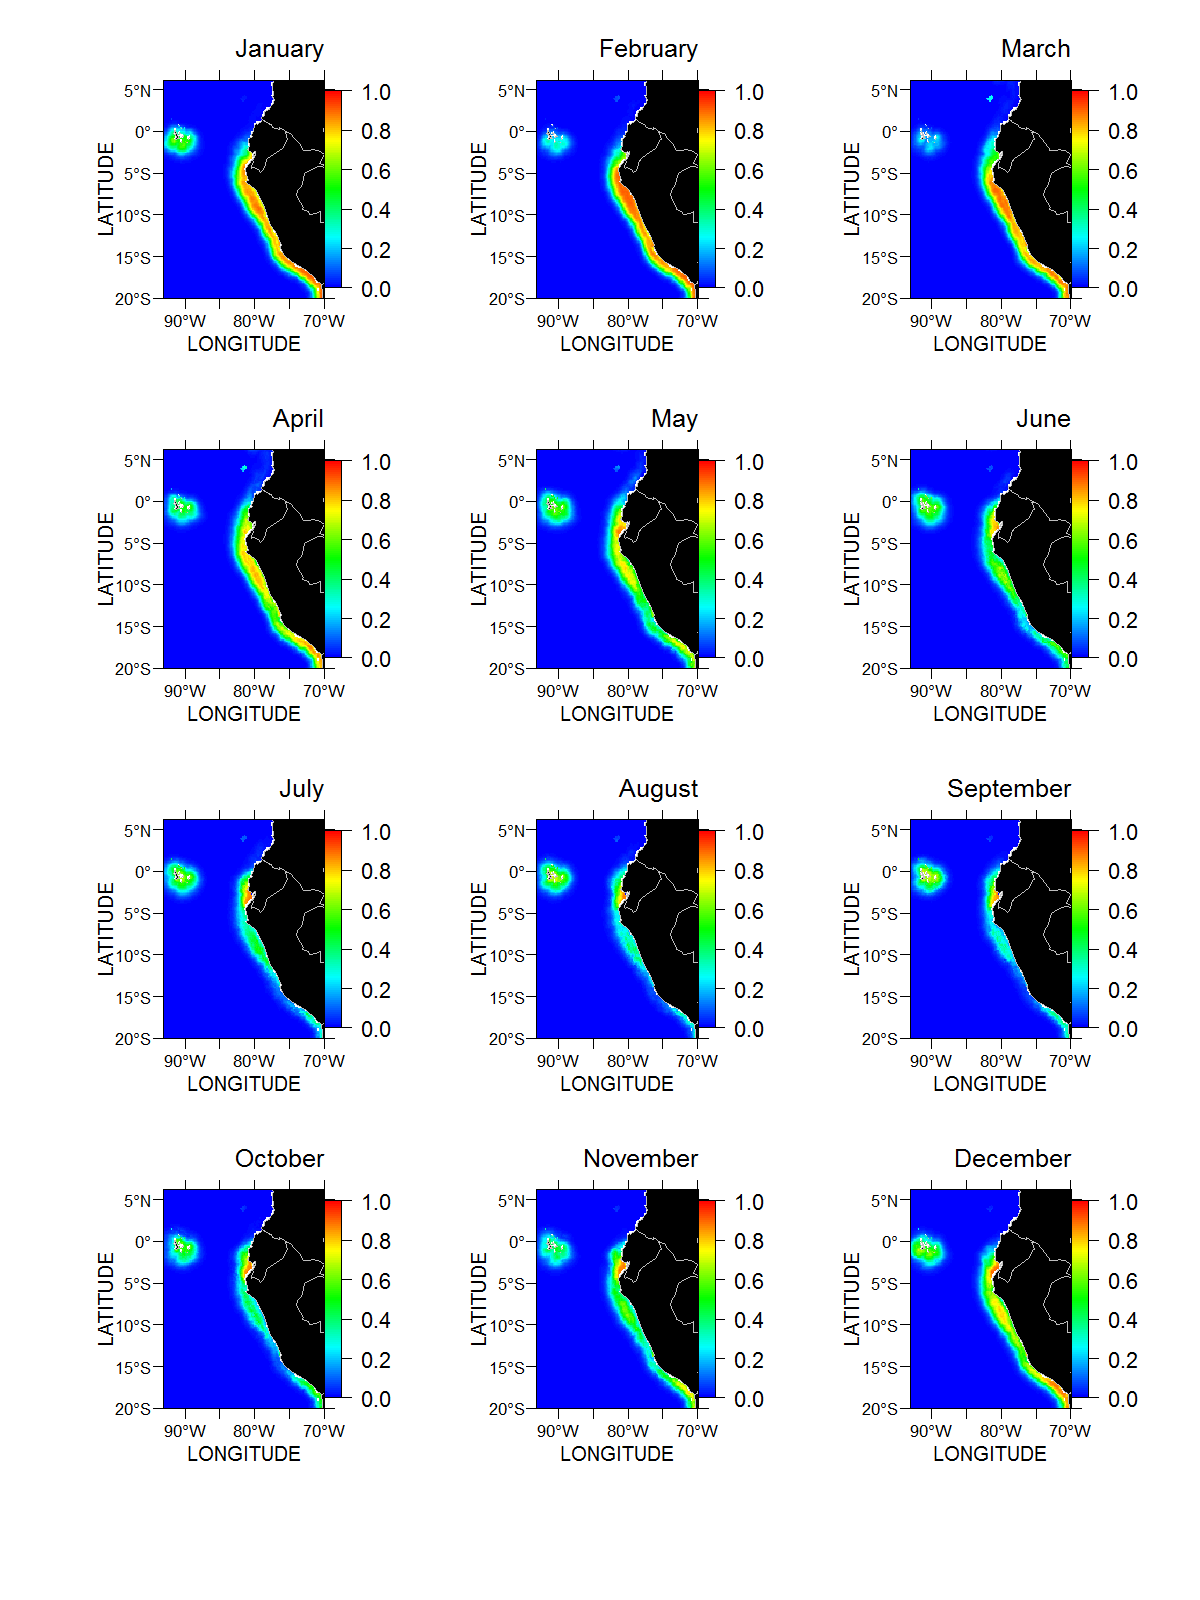
\includegraphics[height=0.8\textheight]{figures/sardine-climatology}
\caption[Seasonal patterns of the distribution of Peruvian anchovy]{Seasonal patterns of the distribution of sardine as predicted by the species distribution models used to build the interannual maps for the NHCE OSMOSE model.}
\label{fig:sardine-climatology}
\end{figure}


\section*{References}

Aumont O. and Bopp L. 2006. Globalizing results from ocean in situ iron fertilization studies. Gl.Biogeochem.Cyc. 20:GB2017.

Budgell, W.P., 2005: Numerical simulation of ice-ocean variability in the Barents Sea region, Ocean Dynamics, DOI 10.1007/s10236-005-0008-3.

Cambon G.,Goubanova K., Marchesiello P., et al. 2013. Assessing the impact of downscaled atmospheric winds on a regional ocean model simulation of the Humboldt system. Ocean Modelling 65:11-24.

Colas, F., X. Capet, J. C. McWilliams, et al. 2008. 1997–1998 El Nino off Peru: A numerical study. Prog. Oceanogr.79:138–155.

Da Silva A.M., Young C.C. Levitus S. 1994. Atlas of surface marina data 1994. Technical report, Natl. Oceanogr. And Atmos. Admin. Silver Spring Md.

Di Lorenzo, E., 2003: Seasonal dynamics of the surface circulation in the southern California Current System, Deep-Sea Res., Part II, 50, 2371-2388.

Dinniman, M. S., J. M. Klinck, and W. O. Smith Jr. (2003), Cross shelf exchange in a model of the Ross Sea circulation and biogeochemistry, Deep-Sea Res., Part II, 50, 3103-3120.

Echevin V., Goubanova K., Dewitte B., A., et al. 2012. Sensitivity of the Humboldt Current system to global warming: a downscaling experiment of the IPSL-CM4 model. Clim. Dyn. 38(3-4):761-774.

Espinoza-Morriberón D. 2012. Impacto de la circulaciónecuatorialen la zonamínima de oxígenopresenteen el nortedelEcosistema de la Corriente de Humboldt.Thesis to obtain the degree of Master in Marine Sciences. Unidad de PostgradoVíctorAlzamora. Facultad de Ciencia y Filosofía. Universidad PeruanaCayetano Heredia, Lima. 115 pp.

Espinoza-Morriberón D., Echevin V., Romero Y.,  Ledesma J., Oliveros-Ramos R., Tam J., (submitted) Validation of ROMS-PISCES Coupled Model in the Southeast Pacific. Part II: Biogeochemical conditions.

Gruber N., Frenzel H., Doney S.C., et al. 2006. Eddy-resolving simulation of plankton ecosystem dynamics in the California Current System. Deep Sea Res. 1(53): 1483-516.

Haidvogel, D. B., H. G. Arango, K. Hedstrom, A. Beckmann, P. Malanotte-Rizzoli, and A. F. Shchepetkin (2000), Model evaluation experiments in the North Atlantic Basin: Simulations in nonlinear terrain-following coordinates, Dyn. Atmos. Oceans, 32, 239-281.

Montes I., Colas F., Capet X., et al. 2010. On the pathways of the equatorial subsurface currents in the eastern equatorial Pacific and their contributions to the Peru Chile Undercurrent. J. Geophys. Res. 115: C09003.

Penven P., Echevin V, Pasapera J, et al. 2005. Average circulation, seasonal cycle, and mesoscale dynamics of the Peru Current System: A modeling approach. J. Geophys. Res. 110: C10021. DOI:10.1029/2005JC002945.

Redfield A.C., Ketchum B.H. and Richards F.A. 1963. The influence of organisms on the composition of the sea-water. En: Hill M.N. (Eds.). Interscience 2: 26-77.

Risien C.M. and Chelton D.B. 2008. A Global Climatology of Surface Wind and Wind Stress Fields from Eight Years of QuikScatscatterometer Data. J. Phys. Oceanogr. 38: 2379-2413.

Romero Y., Espinoza-Morriberón D., Oliveros-Ramos R., Tam J., Echevin V. (submitted) Validation of ROMS-PISCES Coupled Model in the Southeast Pacific. Part I: Physical conditions.

Peliz, A., J. Dubert, D. B. Haidvogel, and B. Le Cann (2003), Generation and unstable evolution of a density-driven Eastern Poleward Current: The Iberian Poleward Current, J. Geophys. Res., 108(C8), 3268, doi:10.1029/2002JC001443.

Shchepetkin, A.F., McWilliams, J.C., 2005. Regional Ocean Model System: a split-explicit ocean model with a free-surface and topography-following vertical coordinate. Ocean Modelling 9, 347-404.

Warner, J.C, C.R. Sherwood, H.G. Arango, and R.P. Signell (2005) Performance of four Turbulence Closure Methods Implemented using a Generic Length Scale Method. Ocean Modelling, 8, 81-113.

Wilkin, J.L., H.G. Arango, D.B. Haidvogel, C.S. Lichtenwalner, S.M. Durski, and K.S. Hedstrom, 2005: A regional Ocean Modeling System for the Long-term Ecosystem Observatory. J. Geophys. Res., 110, C06S91, doi:10.1029/2003JC002218.

